\documentclass{beamer}

% Font selection
\usepackage{palatino}

% Beamer template
\usetheme{Antibes}
%\usetheme{Berlin}

\usepackage[scale=1.2]{ccicons}

\usepackage[utf8]{inputenc}
\usepackage[T1]{fontenc}
\usepackage[spanish]{babel}

\usepackage{tabularx}
\usepackage{multicol}

\usepackage{listings}

\lstset{
  language=C++,
  columns=flexible,
  identifierstyle=\itshape,
%
  belowcaptionskip=1\baselineskip,
  breaklines=true,
  xleftmargin=\parindent,
  language=C++,
  showstringspaces=false,
  basicstyle=\tiny,
  keywordstyle=\bfseries\color{green!40!black},
  commentstyle=\itshape\color{purple!40!black},
  identifierstyle=\color{blue},
  stringstyle=\color{brown},
  columns=flexible,
%  inputenconding=utf8,
  extendedchars=true,
%
  morekeywords=[1]{constexpr,nullptr,alignof,alignas,decltype},
  literate={%
    {¿}{{?`}}1
    {¡}{{!`}}1
    {á}{{\'a}}1
    {é}{{\'e}}1
    {í}{{\'i}}1
    {ó}{{\'o}}1
    {ú}{{\'u}}1
    {ñ}{{\~n}}1
}
}

\newcommand{\cppkey}[1]{%
{\textbf{\color{green!40!black}\texttt{#1}}}%
}

\newcommand{\cppid}[1]{%
{\textbf{\color{blue}\texttt{#1}}}%
}

\lstdefinestyle{terminal}{
  language=bash,
  basicstyle=\scriptsize\ttfamily,
  numbersep=3pt,
  frame=tb,
  columns=fullflexible,
  backgroundcolor=\color{yellow!20},
  literate=%
    {¿}{{?`}}1
    {¡}{{!`}}1
    {á}{{\'a}}1
    {é}{{\'e}}1
    {í}{{\'i}}1
    {ó}{{\'o}}1
    {ú}{{\'u}}1
    {ñ}{{\~n}}1
}


\usepackage{tikz}
\usetikzlibrary{positioning}
\usetikzlibrary{arrows}
\usetikzlibrary{mindmap}

\usepackage{pgfplots}
\pgfplotsset{compat=1.5}



% Footline in every slide
\setbeamertemplate{footline}{
  \leavevmode%
  \hbox{\begin{beamercolorbox}[wd=\paperwidth,ht=2.5ex,dp=1.125ex,leftskip=.3cm,rightskip=.3cm]{author in head/foot}%
    \usebeamerfont{author in head/foot}\ccbyncndeu \quad -- \quad J. Daniel Garcia -- ARCOS@UC3M (\url{josedaniel.garcia@uc3m.es})
    \quad Twitter \url{@jdgarciauc3m}
    \hfill
    \insertframenumber/\inserttotalframenumber
  \end{beamercolorbox}}%
  \vskip0pt%
}

% Logo in every slide
\addtobeamertemplate{headline}{}
{% 
\begin{tikzpicture}[remember picture,overlay]
\node[anchor=north east] at (current page.north east) {
\includegraphics[height=0.7cm]{logos/arcos_t.png}};
\end{tikzpicture}
}

%\addtobeamertemplate{footline}{}
%{% 
%\begin{tikzpicture}[remember picture,overlay]
%\node[anchor=south east,outer ysep=0.8cm] at (current page.south east) {\includegraphics[height=0.7cm]{../logos/techfest.png}};
%\end{tikzpicture}
%}

\tikzset{
  invisible/.style={opacity=0},
  visible on/.style={alt=#1{}{invisible}},
  alt/.code args={<#1>#2#3}{%
    \alt<#1>{\pgfkeysalso{#2}}{\pgfkeysalso{#3}} % \pgfkeysalso doesn't change the path
  },
}

%Portada
\title{C++ en la industria de los videojuegos}
\subtitle{C/C++ Meetup}
\author{J. Daniel Garcia}
\institute{Grupo ARCOS\\Universidad Carlos III de Madrid}
\date{4 de diciembre de 2015}

\begin{document}

\begin{frame}
\titlepage
\end{frame}

\AtBeginSection[]
{
  \begin{frame}<*>
    \setbeamertemplate{section in toc shaded}[default][50]
    \setbeamertemplate{subsection in toc shaded}[default][50]
    \tableofcontents[currentsection,hideallsubsections]
  \end{frame}
}

\AtBeginSubsection[]
{
  \begin{frame}<beamer>
    \setbeamertemplate{subsection in toc shaded}[default][50]
    \tableofcontents[sectionstyle=show/hide,subsectionstyle=show/shaded/hide]
  \end{frame}
}

\begin{frame}{Licencia}

\begin{tabularx}{.98\textwidth}{lX}
\ccLogo & Esta obra está bajo una Licencia Creative Commons Atribución-NoComercial-SinDerivar 4.0 Internacional.\\

\ccAttribution & 
Debes dar crédito en la obra en la forma especificada por el autor o licenciante.\\

\ccNonCommercialEU &
El licenciante permite copiar, distribuir y comunicar públicamente la obra. A
cambio, esta obra no puede ser utilizada con fines comerciales — a menos que se
obtenga el permiso expreso del licenciante.
\\

\ccNoDerivatives &
El licenciante permite copiar, distribuir, transmitir y comunicar públicamente
solamente copias inalteradas de la obra -- no obras derivadas basadas en ella.
\\

\end{tabularx}

\vfill
\begin{footnotesize}
Fuentes disponibles en: \textbf{\color{blue}\url{github.com/jdgarciauc3m/gamespp-2015}}
\end{footnotesize}


\end{frame}

\begin{frame}[t]{Special Thanks}
\begin{itemize}
  \item This talk is based on material provided by Michael Wong (IBM, Chair of SG14).
  \item Thanks also go to many people contributing to SG14.
\end{itemize}
\end{frame}

\begin{frame}[t]{Lo que yo sé de videojuegos}
\pause
\begin{columns}[T]

\column{.5\textwidth}

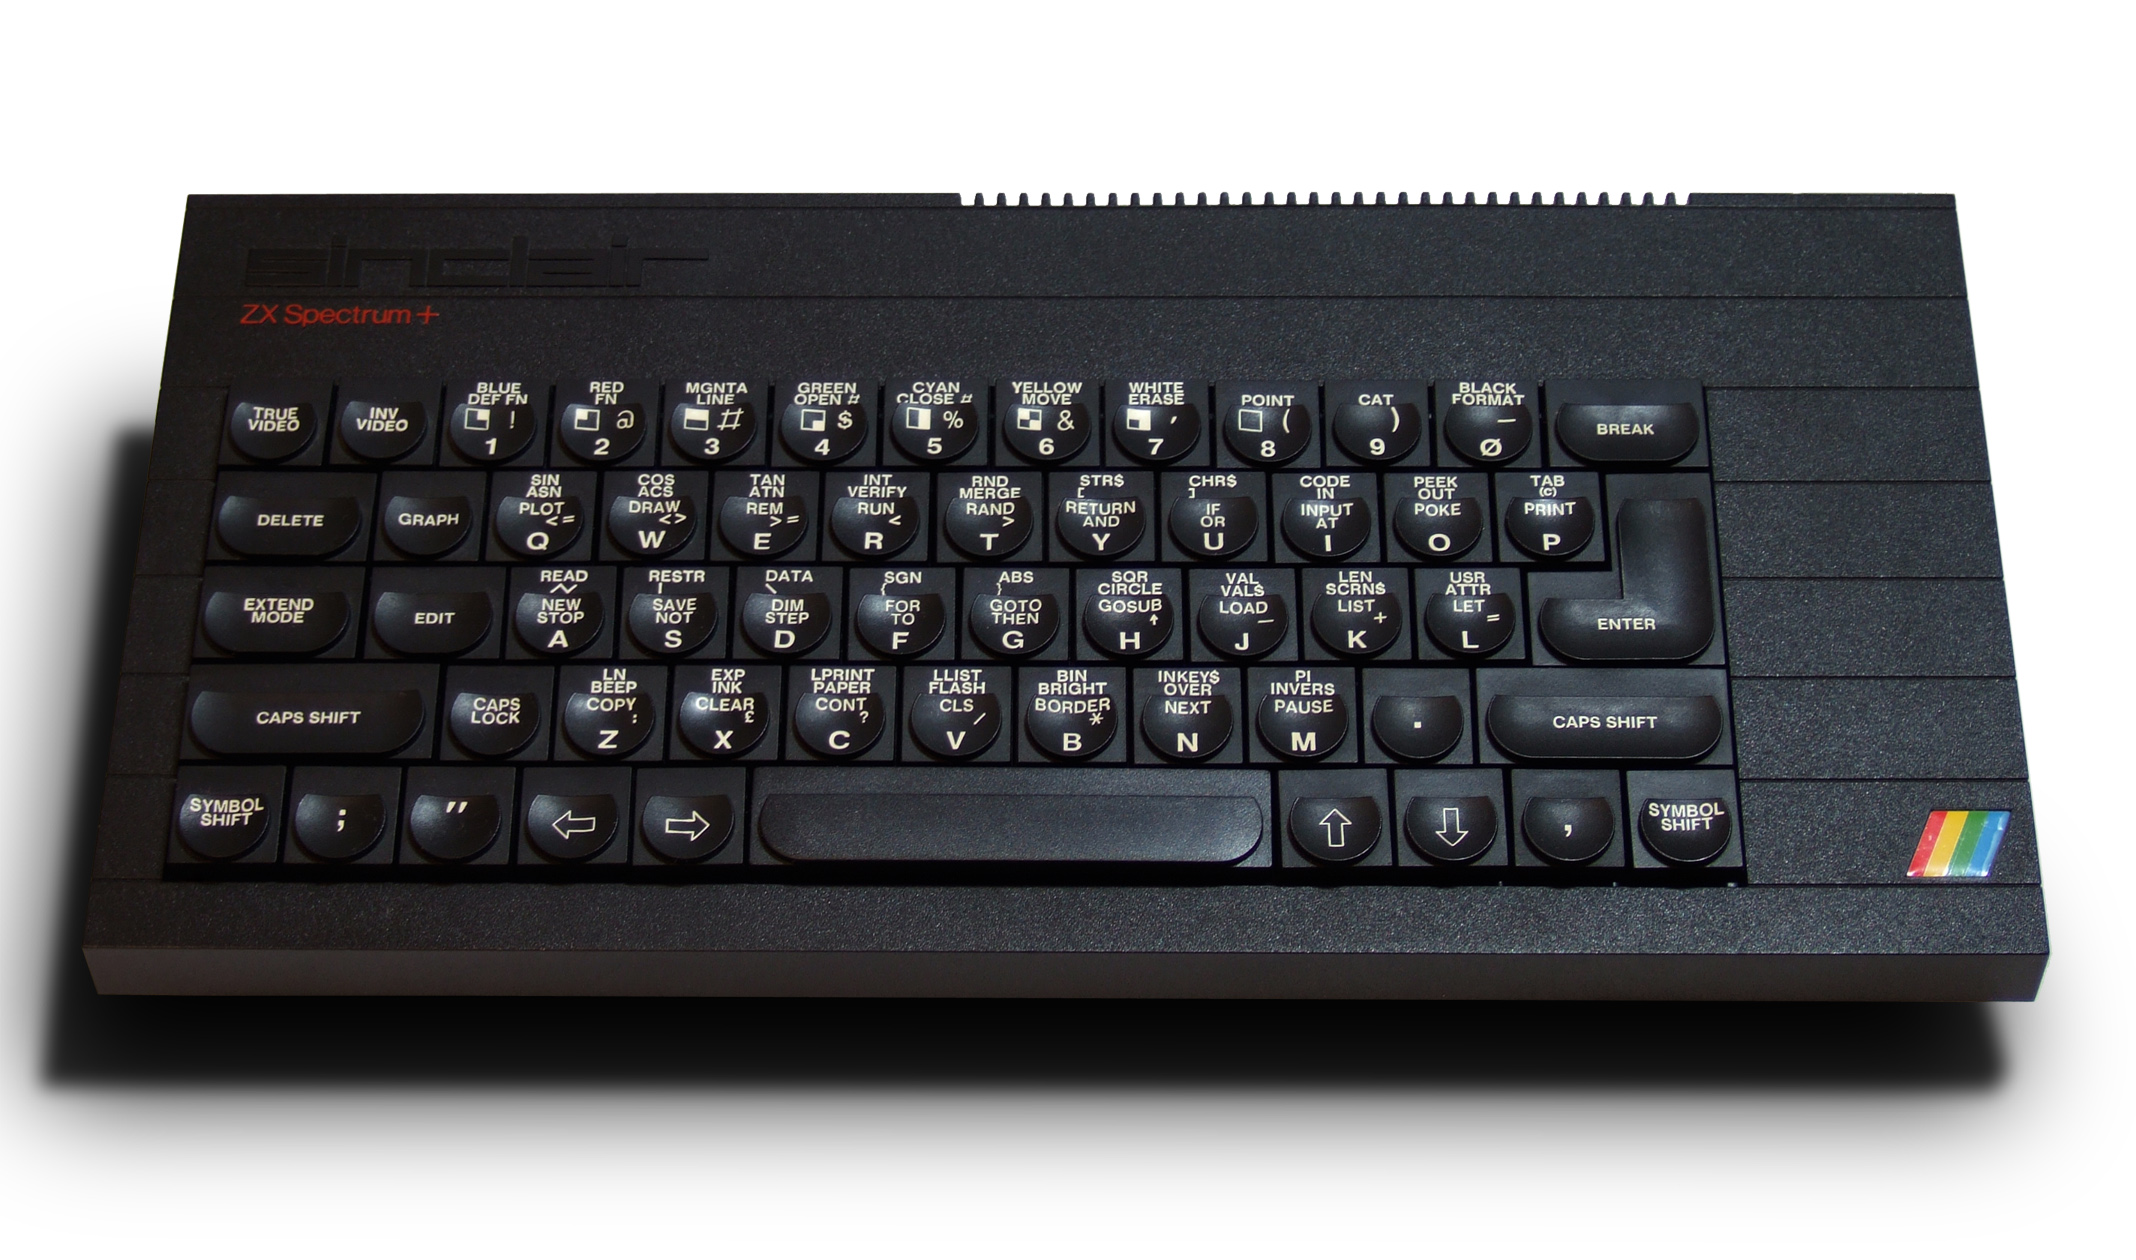
\includegraphics[width=.7\textwidth]{figs/zx-spectrum}
\vspace{1cm}
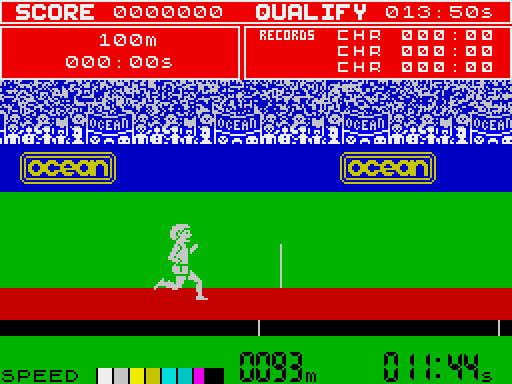
\includegraphics[width=.7\textwidth]{figs/decathlon}

\column{.5\textwidth}


\includegraphics[width=.6\textwidth]{figs/rambo}
\vspace{1cm}
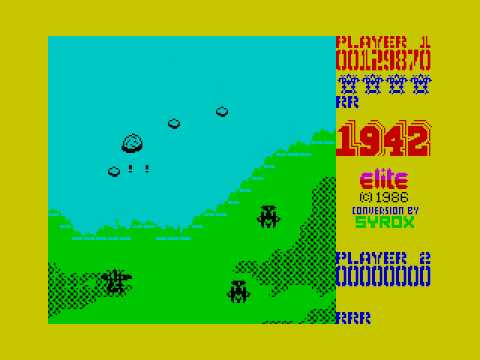
\includegraphics[width=.6\textwidth]{figs/1942}

\end{columns}
\end{frame}

\section{El grupo SG14}

\begin{frame}[t]{C++ y videojuegos}
\begin{columns}

\column{.6\textwidth}
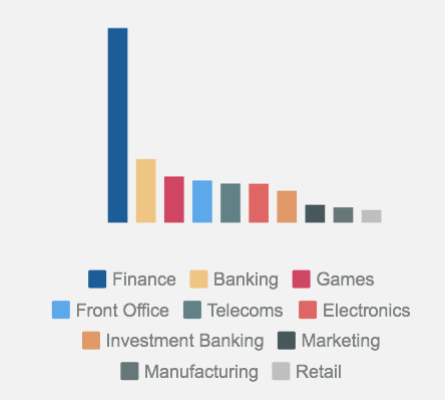
\includegraphics[height=.7\textheight]{figs/clion-market}

\column{.4\textwidth}

\includegraphics[width=4cm]{logos/clion}


\includegraphics[width=4cm]{logos/jetbrains}

\end{columns}
\vfill
{\tiny\color{blue}\textbf{\url{http://blog.jetbrains.com/clion/2015/07/infographics-cpp-facts-before-clion/}}}
\end{frame}

\begin{frame}{El comité de C++}
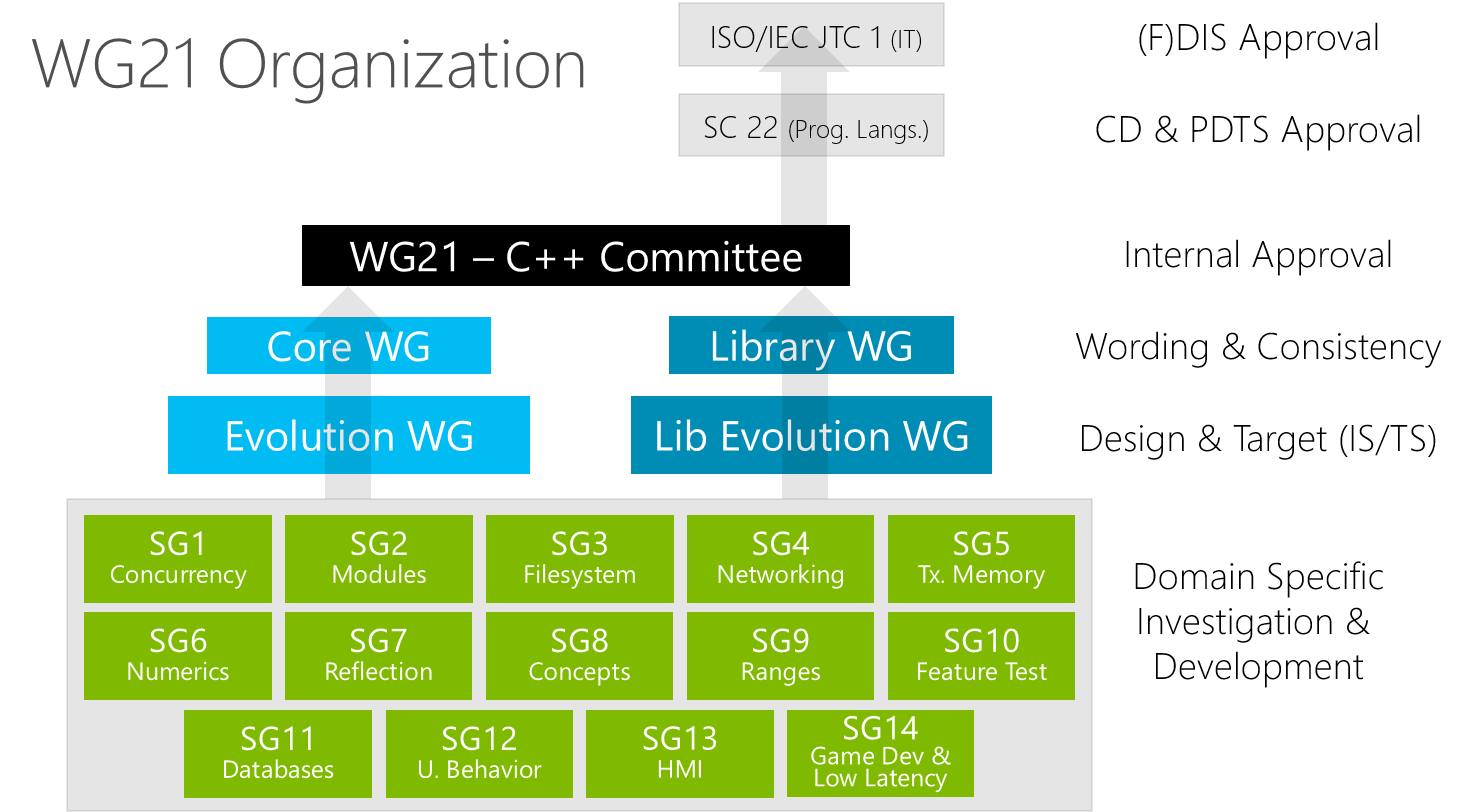
\includegraphics[height=6cm]{figs/sc22-wg21}
\end{frame}

\begin{frame}[t]{Orígenes}
\begin{itemize}
  \item \textbf{CppCon 2014}: Comité se encuentra con desarrolladores.
    \begin{itemize}
      \item Discusiones preliminares.
      \item Lista de correo y grupo en Google Groups.
      \item N4456: Towards improved support for games, graphics, real-time, low latency, embedded systems.
    \end{itemize}
  \vfill\pause
  \item Creación de SG14: \emph{Game Development and Low Latency}
    \begin{itemize}
      \item Chair: Michael Wong (IBM).
      \item Próxima reunión: GDC 2016.
      \item SG14 se reune para enviar propuestas a WG21 (Comité C++).
    \end{itemize}
\end{itemize}
\end{frame}

\begin{frame}[t,shrink=10]{Otros sectores interesados}
\begin{itemize}
  \item Otros sectores atraidos:
    \begin{itemize}
      \item Finnancial/Trading.
      \item Banca.
      \item Simulación.
      \item HPC.
      \item Big Data Analytics?
    \end{itemize}
  \vfill\pause
  \item ¿Por qué?
    \begin{itemize}
      \item Simulaciones interactivas 
        \begin{itemize}
          \item Simulación, software de formación.
        \end{itemize}
      \item Gráficos en tiempo real.
        \begin{itemize}
          \item Simulación, software de formación.
        \end{itemize}
      \item Computación de baja latencia .
        \begin{itemize}
          \item Simulación, software de formación, finanzas, trading.
        \end{itemize}
      \item Recursos restringidos. 
        \begin{itemize}
          \item Sistemas empotrados.
        \end{itemize}
      \item Altas prestaciones 
        \begin{itemize}
          \item Computación científica, Big Data analytics.
        \end{itemize}
    \end{itemize}
\end{itemize}
\end{frame}

\section{Algunos problemas}

\begin{frame}[t]{Memoria}
\begin{itemize}
  \item Memoria disponible.
    \begin{itemize}
      \item Presupuesto de memoria fijo (entre centenares de MB y pocos GB).
      \item Sin espacio de \emph{swap} ni espacio temporal de disco.
      \item \alert{¡Actualizar el hardware no es una opción!}
    \end{itemize}
  \vfill\pause
  \item Inconsistencias en asignación de memoria.
    \begin{itemize}
      \item Diferencias en implementaciones de contenedores.
        \begin{itemize}
          \item Tasa de crecimiento de vector, tamaño inicial, optimización del objeto pequeño, \ldots
        \end{itemize}
      \item ¿A partir de qué tamaño se requiere asignación en \cppid{std::function}?
      \item Consecuencia: Problema de \alert{portabilidad de rendimiento}.
    \end{itemize}
\end{itemize}
\end{frame}

\begin{frame}[t]{Tiempo de cómputo}
\begin{itemize}
  \item Coste de iteradores en versiones de \emph{debug}.
    \begin{itemize}
      \item Variable entre implementaciones.
      \item Diferentes formas de desactivar características no deseadas.
    \end{itemize}
  \vfill\pause
  \item \cppid{dynamic\_cast} normalmente desactivado.
    \begin{itemize}
      \item Sistemas de reflexión \emph{ad-hoc}.
    \end{itemize}
  \vfill\pause
  \item Algoritmos $O(log n)$ con rendimiento variable.
    \begin{itemize}
      \item \cppid{boost::flat\_map} frente a \cppid{std::map}.
    \end{itemize}
\end{itemize}
\end{frame}

\begin{frame}[t]{Rendimiento}
\begin{itemize}
  \item RTTI.
    \begin{itemize}
      \item Overhead de datos generados.
      \item \cppkey{-fno-rtti}.
      \item Uso de \cppkey{dynamic\_cast} $\rightarrow$ \alert{comportamiento no definido}.
    \end{itemize}
  \vfill\pause
  \item Excepciones.
    \begin{itemize}
      \item Restringe optimizaciones (\emph{stack undwinding}).
      \item \cppkey{-fno-exceptions}.
      \item Uso de \cppkey{try} o \cppkey{throw}  $\rightarrow$ \alert{comportamiento no definido}.
      \item Hace muchas bibliotecas inutilizables.
    \end{itemize}
\end{itemize}
\end{frame}

\begin{frame}[t]{Más rendimiento}
\begin{itemize}
  \item Hardware con predicción de salto inexistente (o malo).
  \item El impacto de la caché sobre el rendimiento se hace más visible.
  \item El rendimiento es relevante incluso en depuración.
  \item Estructuras de datos.
    \begin{itemize}
      \item Listas enlazadas intrusivas.
      \item Tablas \emph{hash} que sean \emph{cache friendly}.
      \item \ldots
    \end{itemize}
  \item El tiempo importa.
    \begin{itemize}
      \item Tiempos de compilación largos.
      \item Tiempos de carga largos.
    \end{itemize}
\end{itemize}
\end{frame}

\section{Primeras soluciones}

\begin{frame}[t]{Aritmética de coma fija}
\begin{itemize}
  \item Propuestas:
    \begin{itemize}
      \item P0037R0: Fixed point real numbers.
      \item N3352: C++ Binary Fixed-Point Arithmetic.
    \end{itemize}
  \vfill
  \item Razones:
    \begin{itemize}
      \item Plataformas con coma flotante lenta.
      \item Necesidad de precisión uniforme (IEEE 754 tiene precisión variable).
    \end{itemize}
  \vfill
  \item Se propone:
    \begin{itemize}
      \item \cppid{std::fixed\_point<Rep,Exp>}
      \item \cppid{std::make\_fixed<IntBits,FracBits>}
    \end{itemize}
\end{itemize}
\end{frame}

\begin{frame}[t]{Búfer circulares}
\begin{itemize}
  \item Propuesta:
    \begin{itemize}
      \item P0059R0: Add rings to the Standard Library.
      \item Un búfer FIFO contiguo en memoria.
    \end{itemize}
  \vfill
  \item Posibles usos:
    \begin{itemize}
      \item Paso de muestras de audio a DAC.
      \item Cola de paquetes de red pendientes de envío.
      \item Búfer con \emph{frames} de video.
    \end{itemize}
  \vfill
  \item Se propone:
    \begin{itemize}
      \item \cppid{std::fixed\_ring<T,N>}
      \item \cppid{std::dynamic\_ring<T>}
    \end{itemize}
\end{itemize}
\end{frame}

\begin{frame}[t]{Soporte a concurrencia}
\begin{itemize}
  \item Una versión \emph{thread-safe} de la STL.
    \begin{itemize}
      \item En estudio.
    \end{itemize}
  \item Control del tamaño de pila de un \cppid{thread}.
    \begin{itemize}
      \item Necesidad de controlar el tamaño de pila de hilos creados.
      \item Necesario establecer \alert{antes} de crear hilo $\rightarrow$ \cppid{native\_handle()} no sirve.
    \end{itemize}
\end{itemize}
\end{frame}

\begin{frame}[t]{Otras cosas}
\begin{itemize}
  \item Mejores herramientas para implementar contenedores de alto rendimiento.
    \begin{itemize}
      \item Algoritmos sobre almacenamiento \emph{raw}.
      \item Movimiento y construcción sobre memoria no iniciada.
      \item Algoritmos de eliminación no estable.
    \end{itemize}
  \item Contenederos asociativos \emph{``planos''}.
  \item Poder identificar si una instancia tiene una función en su \emph{v-table}.
  \item Coste de las excepciones.
  \item Vistas atómicas.
  \item Más \cppkey{noexcept}.
  \item Mejor SIMD.
  \item \ldots
\end{itemize}
\end{frame}



\begin{frame}
\titlepage
\end{frame}

\end{document}
